% !TEX root = ../thesis.tex
\chapter{Model selection}
\label{capitolo5}
\thispagestyle{empty}

In this chapter we will show the choices and stages behind the final model.
Starting from baseline models, we enhanced the chosen classifiers with handcrafted features coming from the last chapter.\\
We saw and studied the performance improvements with validation approaches, and this phase led us to our current solution.

The result involves three models:
\begin{itemize}
	\item[\PencilRight] a first Random Forest classifier that has been used to provide an early filter on the separation between Genuine accounts and Bots
	\item[\PencilRight] a second Random Forest that gives a classification among the five studied categories
	\item[\PencilRight] a Naive Bayes classifier, used over the same classes of the second Random Forest, but it reads and labels the users, according on their tweets only
\end{itemize}
All the above mentioned algorithms were combined with a stacking ensemble methods, after considering different possibilities.

\section{Baselines}
The choices explained in this section were made at the same time of the ones listed in the Baseline section of the last chapter.

This is, basically, the same stage of the above-mentioned, but in a model-driven perspective.
The features involved are the ones described in that chapter, but we started from that base, to try different classifiers over it.
Each classifier has been fitted with the entire dataset, but considering only baselines features.

Furthermore, no parameters tuning has been applied, in order to minimize the results of our baselines classifier, with their standard assets.
\subsection{Random Forest}
Random forest is an ensemble learning method used in classification tasks and prediction ones as well.

The algorithm builds several \textit{decision trees} and the resulting output is provided by the mode of the predictions coming from the estimators in the forest.

Each decision tree is trained on a subset of the original data, formed by sampling with replacements the whole training set. They share the same splitting criterion, in order to build subtrees, which is the entropy:\\
Every tree computes the Information Gain of each feature, which is the difference, in terms of entropy, between the information gained on the data \textit{D}, before splitting on the attribute \textit{X}, and the one gained after the split, which provides \textit{n} subsets of \textit{D}.
\[{ \mathit{InformationGain(X)} = \mathit{Information(D)} - \mathit{Information_{X}(D)}}\]
where
\[{ \mathit{Information(D)} = - p_{1}\log p_{1} - ... - p_{n} \log p_{n}}\]
and
\[{ \mathit{Information_{X}(D)} = \frac{|D_{1}|}{|D|}Information(D_{1}) + ... + \frac{|D_{n}|}{|D|}Information(D_{n}) }\]
The attribute providing the highest InformationGain, against the others at the same level of the tree, is chosen to perform a split.

The feature set considered by each tree is a random subset of the original pool.

Due to its ability to face overfitting and to the feature importance ranking that it can provide, this tool is often preferred over other models belonging to the same category.

The advantage of preventing overfitting usually comes with a slower prediction time, because it needs enough estimators for this task.
But, for our purpose, there were enough estimators to face the variance problem without affecting the generalization speed.
\subsection{Logistic Regression}
Logistic regression is a common statistical model, that uses a sigmoid function to map the output of a linear regression on a normalized score, giving the probability, for each sample, to belong to the positive class, given its features and a weighting vector:
\[{\displaystyle P(\hat{y}_{i} = +1 | \vec{x}_{i}, \vec{w})={\frac {1}{1+e^{-\vec{w}h(\vec{x}_{i})}}}}\]

Where $ \hat{y}_{i} $ is the predicted target, over the  \textit{$i_{th}$} sample, \textit{$ \vec{x}_{i} $} is the feature vector of that sample, \textit{$ \vec{w} $} represents the weighting vector that has to be learned and \textit{h} is the activation function of the linear regression.

Logistic Regression searches for the weighting vector that matches the highest likelihood and, in order to do that, it minimizes a cross-entropy
error function, provided by the negative log of the likelihood:
\[{ \mathbf{L}(\vec{w}) = -\ln \prod\limits_{i=1}^{n} P(\hat{y}_{i} = +1 | \vec{x}_{i}, \vec{w})}\]

In multiclasses tasks, there are two possible approaches to face the problem:
\begin{itemize}
	\item[\PencilRight] a more general \textit{softmax} function to replace the logistic sigmoid, which assigns the probability, for the  \textit{$i_{th}$} sample, to belong to the class \textit{C}:
	\[{\displaystyle P(\mathbf{C}_{i} | \vec{x}_{i}, \vec{w})={\frac {e^{-\vec{w}h(\vec{x}_{i})}}{\sum\limits_{j = 1}^{n}e^{-\vec{w}h(\vec{x}_{j})}}}}\]
	\item[\PencilRight] "One-vs-Rest" method, which for each class, it builds a model that predicts the target class against all the others.
\end{itemize}
We decided to stick with the default settings of the libraries involved, so OvR was the approach used for the baseline.

\subsection{K-Nearest Neighbors}
K-Nearest Neighbors is an instance-based model used for classification, regression and pattern recognition. It is considered as a lazy learning algorithm, because all the computation is deferred until the prediction phase.
When it performs a classification over a new point, it looks for the \textit{K} nearest samples in the training set, according to a chosen metric, and it assigns, to the unseen sample, the mode of the targets of the retrieved neighbors.

The choices to make are the ones regarding the number \textit{K} of neighbors to consider, the weights to assign to them and the metric to calculate the distance with.
We used the default settings for the metric (\textit{Euclidean distance}) and for the weighting technique (\textit{uniform}), but we chose to consider 10 neighbors, because the automatic setting was \textit{K} = 5, which is the number of our possible targets.
We chose a \textit{K} that is large enough to make the model not too sensible to outliers, and restricted enough to sharpen the classes boundaries.

We first normalized the training data and then we fitted the algorithm on them, in order to simplify the distance computations.

\subsection{Support Vector Machine}
Support Vector Machine is a smart way to do instance-based learning. It can be seen as a generalization of the weighted KNN algorithm, with an arbitrary and feasible \textit{kernel function}, instead of the more generic dot product.

It can be summarised with a support vector $ \mathbf{\vec{x}} $ (a subset of the training set), a weighting vector $ \mathbf{\vec{w}} $ for them and a \textbf{kernel} \textit{K(x, x')} (a similarity function).

In order to make it work properly, three choices must be made:
\begin{itemize}
	\item[\PencilRight] a proper kernel, which is often selected according to experience and domain knowledge of the problem. We wanted to make things simple in this stage, so we used the default kernel function, which is the Radial Basis Function:
	\[ K(x, x') = exp(- \frac{||x-x'||^{2}}{2\sigma^{2}}) \]
	with $ \sigma $ as a free parameter
	\item[\PencilRight] the weights $ \vec{w} $, which are obtained by maximizing the margin that splits the records belonging to different classes. Each samples are mapped into a space, thanks to what is known as the \textit{kernel trick}. The "trick" helps a linear classifier to work on a non-linear problem, applying the kernel function in the prediction phase.\\This process highlights the boundary that separates the points belonging to different classes.
	SVM aims to draw the boundary for the classes, in order to maximize the "margin" formed between the closest points that have different targets
	\item[\PencilRight] the support vector $ \vec{x} $, which comes as a consequence of choosing weights
\end{itemize}
Since we were still facing a multitarget problem, the binary nature of SVM must had been adapted to our needs. We decided, once again, to stick with the default setting for non-binary classifications, in order to have only raw baselines to compare.

The multitarget classification is handled with "One-vs-One" approach.
It considers all possible pairwise binary classifiers and so it leads to $\frac{N(N-1)}{2}$ individual binary classifiers, where N is the number of the classes in the problem.

In comparison with "One-vs-Rest" approach, "One-vs-One" is less sensitive to an imbalanced dataset, but it's more computationally expensive then the the other, which only builds N binary classifiers.
Despite our choices over methods and parameters weren't accurate in this stage as they were in the other ones, we decided to stick with this setting for SVM, because otherwise it would have led us to an irrelevant algorithm, in comparison with the above-mentioned.

\subsection{Comparison and baseline selection}
The selected baseline models were tested with a holdout approach at first, then with a crossvalidation method.
We built a Confusion Matrix for each model, in order to bring out goodness indices for each class, such as \textit{True Positive} (TP), \textit{False Positive} (FP) and \textit{False Negative} (FN).
The evaluation metrics considered are \textit{Precision}, \textit{Recall} and \textit{F1 score} and they work on the mentioned indices.
\begin{itemize}
	\item[\PencilRight] $ Precision = \frac{TP}{TP+FP} $\\
	It measures the proportion of positive identifications, for a given target, that was actually correct
	\item[\PencilRight] $ Recall = \frac{TP}{TP+FN} $\\
	It measures the proportion of actual positive classifications that was identified correctly
	\item[\PencilRight] $ F1 score = \frac{2(Precision \times Recall )}{Precision+Recall} $\\
	It calculates the harmonic mean of the previous metrics
\end{itemize}
Every metric is adapted to fit a multiclass problem. For each class, it has been computed this set of measures, and then they were averaged without weights (macro average), in order to not take label imbalance into account.

The results are pretty similar between the two methods, however we used the one coming from crossvalidation to select the model to build.
\subsubsection{Holdout evaluation}
The holdout stage is performed separating the samples in the dataset into training and test subsets. The splitting process is randomized, and we decided to use the 75\% of the data for the training set and the 25\% for the test set. This choice is a little bit different from the most common one, which builds the training set with 2/3 of the whole data, because we didn't dispose of a huge amount of records, so we preferred this ratio and then trying an other validation method for comparison.
Here we list the algorithm and their parameters, as they were written according to the Scikit-learn library for Python, their confusion matrix and their scores:
\begin{itemize}
	\item[\PencilRight] \textit{RandomForestClassifier(n\_estimators = 10, criterion = 'entropy')}\\
	Confusion matrix:
	
	{
		\centering
		\begin{tabular}{@{}cc|ccccc@{}}
			\multicolumn{1}{c}{} &\multicolumn{1}{c}{} &\multicolumn{5}{c}{Predicted class} \\ 
			\multicolumn{1}{c}{} & 
			\multicolumn{1}{c|}{} & 
			\multicolumn{1}{c}{NSFW} & 
			\multicolumn{1}{c}{NS} &
			\multicolumn{1}{c}{SB} & 
			\multicolumn{1}{c}{FF} & 
			\multicolumn{1}{c}{GEN}\\
			\cline{2-7}
			\multirow[c]{5}{*}{\rotatebox[origin=tr]{90}{Actual class}}
			& NSFW  & 1654 & 23 & 14 & 4 & 68\\
			& NS  & 30 & 716 &  31 &  3 & 81\\
			& SB  & 6 &  27 & 1223  &   3  & 53\\
			& FF  & 15  &  4  &   6  & 1212  &  3\\
			& GEN  & 67 &  74   & 45  &   3 & 718 \\
			\cline{2-7}\\
		\end{tabular}\\
	}
	
	Precision: 0.895\\
	Recall: 0.894\\
	F1 score: 0.894

	\item[\PencilRight] \textit{LogisticRegression(fit\_intercept=True, max\_iter=100, penalty='l2')}\\
	Confusion matrix:
	
	{
		\centering
		\begin{tabular}{@{}cc|ccccc@{}}
			\multicolumn{1}{c}{} &\multicolumn{1}{c}{} &\multicolumn{5}{c}{Predicted class} \\ 
			\multicolumn{1}{c}{} & 
			\multicolumn{1}{c|}{} & 
			\multicolumn{1}{c}{NSFW} & 
			\multicolumn{1}{c}{NS} &
			\multicolumn{1}{c}{SB} & 
			\multicolumn{1}{c}{FF} & 
			\multicolumn{1}{c}{GEN}\\
			\cline{2-7}
			\multirow[c]{5}{*}{\rotatebox[origin=tr]{90}{Actual class}}
			& NSFW  & 1310 & 176 &  78 &   40 & 159\\
			& NS  & 26 & 676 &  54 &  1 & 104\\
			& SB  & 25 &  60 & 947 &  221  & 59\\
			& FF  & 167 &  27  & 11 & 1032 &   3\\
			& GEN  & 118 & 295 & 172  &   8 & 314 \\
			\cline{2-7}\\
		\end{tabular}\\
	}
	
	Precision: 0.675\\
	Recall: 0.685\\
	F1 score: 0.673
	
	\item[\PencilRight] \textit{KNeighborsClassifier(n\_neighbors=10)}\\
	Confusion matrix:
	
	{
		\centering
		\begin{tabular}{@{}cc|ccccc@{}}
			\multicolumn{1}{c}{} &\multicolumn{1}{c}{} &\multicolumn{5}{c}{Predicted class} \\ 
			\multicolumn{1}{c}{} & 
			\multicolumn{1}{c|}{} & 
			\multicolumn{1}{c}{NSFW} & 
			\multicolumn{1}{c}{NS} &
			\multicolumn{1}{c}{SB} & 
			\multicolumn{1}{c}{FF} & 
			\multicolumn{1}{c}{GEN}\\
			\cline{2-7}
			\multirow[c]{5}{*}{\rotatebox[origin=tr]{90}{Actual class}}
			& NSFW  & 1512 &  39  &  50  &  82 &  80\\
			& NS  & 46 & 674  &  28  &  14  & 99\\
			& SB  & 45 &  24 & 1077  &  38 & 128\\
			& FF  & 88  &  4  &  94 & 1018  & 36\\
			& GEN  & 138 &  69  & 132  &  86 & 482\\
			\cline{2-7}\\
		\end{tabular}\\
	}
	
	Precision: 0.769\\
	Recall: 0.762\\
	F1 score: 0.765
	
	\item[\PencilRight] \textit{SVC(kernel='rbf', decision\_function\_shape='ovo')}\\
	Confusion matrix:
	
	{
		\centering
		\begin{tabular}{@{}cc|ccccc@{}}
			\multicolumn{1}{c}{} &\multicolumn{1}{c}{} &\multicolumn{5}{c}{Predicted class} \\ 
			\multicolumn{1}{c}{} & 
			\multicolumn{1}{c|}{} & 
			\multicolumn{1}{c}{NSFW} & 
			\multicolumn{1}{c}{NS} &
			\multicolumn{1}{c}{SB} & 
			\multicolumn{1}{c}{FF} & 
			\multicolumn{1}{c}{GEN}\\
			\cline{2-7}
			\multirow[c]{5}{*}{\rotatebox[origin=tr]{90}{Actual class}}
			& NSFW  & 1761 & 0 &   1  &  0 & 1\\
			& NS  & 861 &  0 & 0 &   0 &  0\\
			& SB  & 1068 & 0 & 244  &  0 & 0\\
			& FF  & 449  & 0 &  0 & 791 & 0\\
			& GEN  & 907 &  0  & 0  &  0 & 0\\
			\cline{2-7}\\
		\end{tabular}\\
	}
	
	Precision: 0.468\\
	Recall: 0.364\\
	F1 score: 0.321
	
\end{itemize}
\subsubsection{Crossvalidation}
This approach is based on repeated holdouts. It is performed by splitting the whole data in \textit{K} non-overlapping folds, leading to \textit{K} different holdout evaluations. The results for each step are stored and the final evaluation is given by the mean of the \textit{K} evaluations. For each evaluation, one fold is used for testing, the other ones for training the models. A common practice is to set \textit{K = 10} and thus averaging 10 different evaluations.
This method is also known as \textit{K-fold crossvalidation}. We used a stratified approach, which takes care about keeping the labels balanced on each fold.

Due the need of performing ten steps, it is computationally more expensive then a simple holdout validation. In our case, it was feasible, in term of speed, because of the models complexity and the data amount.

The obtained scores are also more meaningful, with regards to holdout, because they are less sensitive to "lucky" or "unlucky" splits.

Here is the results for every baseline model:

\begin{itemize}
	\item[\PencilRight] \textit{RandomForestClassifier(n\_estimators = 10, criterion = 'entropy')}\\
	Mean precision: 0.895\\
	Mean recall: 0.891\\
	Mean f1 score: 0.890
	\item[\PencilRight]\textit{LogisticRegression(fit\_intercept=True, max\_iter=100, penalty='l2')}\\
	Mean precision: 0.729\\
	Mean recall: 0.704\\
	Mean f1 score: 0.707
	\item[\PencilRight]\textit{KNeighborsClassifier(n\_neighbors=10)}\\
	Mean precision: 0.785\\
	Mean recall: 0.763\\
	Mean f1 score: 0.764
	\item[\PencilRight]\textit{SVC(kernel='rbf', decision\_function\_shape='ovo')}\\
	Mean precision: 0.443\\
	Mean recall: 0.364\\
	Mean f1 score: 0.314
\end{itemize}

As the results show, the random forest algorithm is the one that achieves the best performances, even with default settings, on both holdout and 10-fold crossvalidation. We thus decided to consider it as the main tool to build our solution. 

\section{Multiclass classifier}
This is the first algorithm involved in our final model.\\
It somehow represents the core of our thesis, it models the starting idea: go deep inside bot identification and search and classify similar behaviours among them.

We started from the baselines identified earlier and we tried to refined them, adjusting to fit our need.

The workflow was the same as before, starting from the data with basis and handcrafted features, we took the best looking algorithm from the baselines pool and performed hyperparameters tuning on it, supported by a validation technique.
\subsection{Dataset}
During this phase, we used the previously described dataset\ref{sec:dataset} with its five different labels.
The algorithm was fed with 26,357 samples and 38 features. the amount of records were light enough to consider K-fold crossvalidation, without slow the validation down too much.
\subsection{Model}
We found ourselves in the situation in which we had some brand new features and we didn't know how useful they were. Obviously, we could appeal to heathmaps or other tools, to highlight the correlations among variables and targets.
However, the model we wanted to develop was the Random Forest, which proved to perform well with F1 score. Since this kind of model exploits its criteria to employ the features, we needed to prove them with a direct approach.

A useful advantage of the Random Forest algorithm is the ability to provide a feature ranking, according to its splitting criterion.
We retrieved the 12 most important attributes, in order to see if we would have found some of the ones coming out from feature engineering.
The algorithm ranking ranked the features this way: 1. \textit{favourites\_count} (0.199402), 2. \textit{followers\_count} (0.110830), 3. \textit{statuses\_count} (0.100810), 4. \textit{avg\_len} (0.058260), 5. \textit{freq} (0.055419), 6. \textit{friends\_count} (0.043405), 7. \textit{ret\_perc} (0.039126), 8. \textit{tweet\_intradistance} (0.033718), 9. \textit{max\_ret} (0.030654), 10. \textit{min\_len} (0.029731), 11. \textit{NSFW\_words\_score} (0.029323), 12. \textit{default\_profile} (0.022897).

\begin{figure}[htp!]
	\centering
	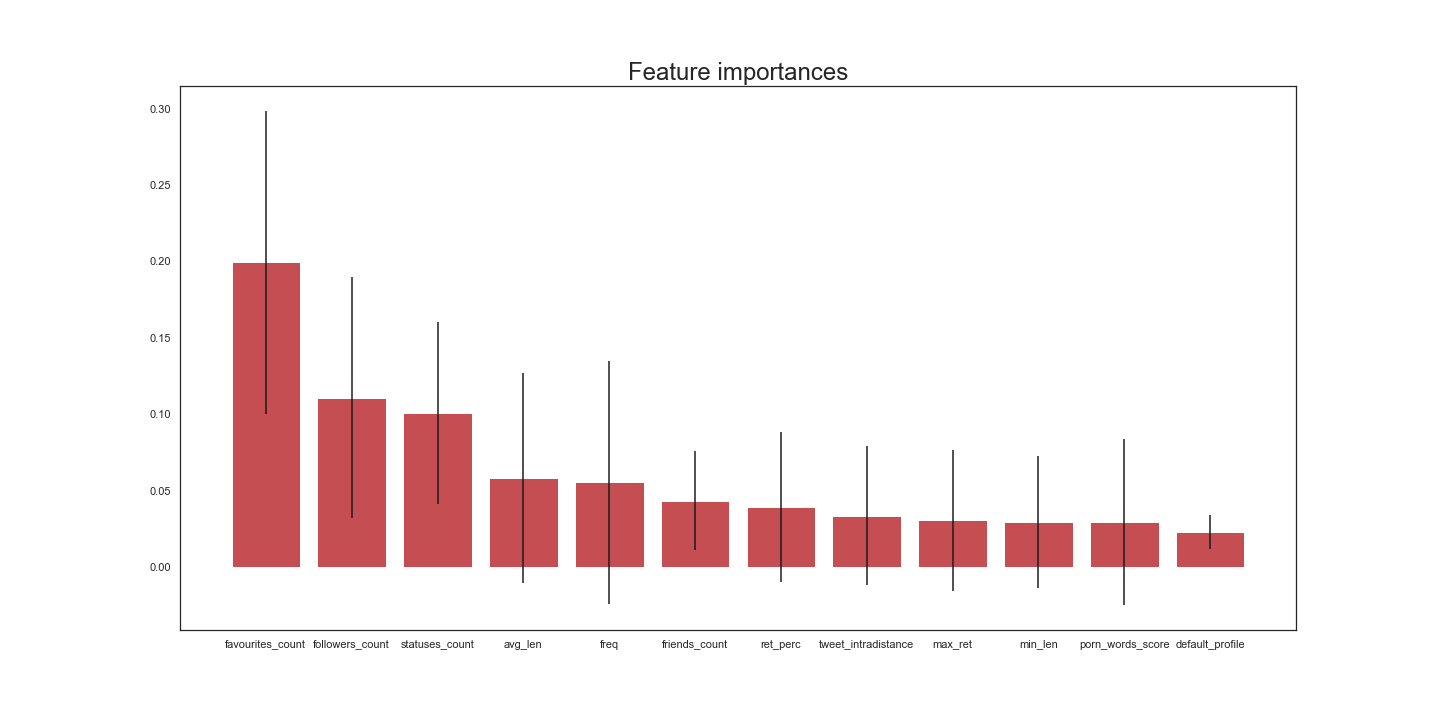
\includegraphics[width=\columnwidth]{chapter5/figure/feature_importances.png}
	\caption{Random Forest feature ranking}
	\label{fig:feature_rank}
\end{figure}

As Figure \ref{fig:feature_rank} shows, we could find some of our crafted features inside this list: lots of tweets descriptive features (\textit{avg\_len, freq, ret\_perc}, etc...), as well as the \textit{tweet\_intradistance} attribute and the \textit{NSFW\_words\_score}.
This picture confirmed us that the idea behind those features was useful.

Since those attributes were thought to belong to different clusters, we decided to try several combinations of those feature clusters, validating the model on them with a crossvalidation. The purpose of this stage was to see if some groups of features were enough to describe the real problem, or if some group would shown up as irrelevant.

Due to the multiclass nature and some imbalances with the labels, we decided to follow the F1 score metric to asses the value of our model.
The crossvalidation was set with 10 folds, as for the baselines tests.
In order to try different hyperparameter assets, we set up a \textit{Grid Search}, using the homonymous function of the Scikit-learn library for Python.
Basically, this method allowed us to define value ranges for the desired hyperparameters, and it permuted all the possible combination of them, returning the associated metric scores.
We wanted to play with the number of trees in the forest, the maximum depth reachable by each tree and the splitting criterion.


\section{Binary Classifier}
Since our dataset was pretty balanced and we couldn't retrieve much more genuine accounts, we didn't want our instruments to treat this category of users just as one the other bot kinds. It was important to perform a previous filter that was able to give importance to the separation between bots and genuine accounts.

We was inspired by the work made with Botometer\cite{Botometer}, which involved a binary labelled dataset, with bot and genuine accounts.
They built their features, grouped them in six main categories, then they ran a Random Forest algorithm per group.

We already had our feature engineering done, so we decided to test it on this new task.

In order to not to build a poorer version of our multiclass model, we didn't want to use a reduced copy of our dataset, stratifying it by stripping random bots from it. We needed a balanced dataset, with about the same amount of genuines and bots. So, we had to gather more human ids, because if we would have relied on the accounts we already had (3661), we would had disposed on a training set with about 7000 entries, that would have been too small to perform a relevant filter.
\subsection{Dataset}
The dataset we used for this classification was composed by part of our collected records and by some entries from the Carvelee-2011 dataset, which contains 22,223 content polluters and 19,276 legitimate users, both collected through a social honeypot, as described in their paper\cite{Lee11sevenmonths}.
This dataset has been involved to build Botometer as well, but we decided to use it only partially, mixing it with our retrieved accounts.

We setted the APIs to retrieve up tu 6,000 ids for both genuines and bots, from the Carvelee list. The process provided us 5,161 legitimate user ids, and 5,297 general bot ids (without inner classifications), because some accounts have been deleted in time.
Then we added some new records, randomly sampling our data. This led us to reach 7,660 human accounts and 7,795 bots, forming a new dataset of 15,455 entries, with binary target.
\subsection{Model}
Since the different purpose of this model, we couldn't rely on the above-mentioned baselines. We wanted to evaluate new raw algorithms for this binary classification.
Another round of crossvalidation with default settings was performed on this new dataset, exploiting the binary nature to show the \textit{Area Under the Curve} score (AUC).
Area Under the Curve represents the goodnes of a classifier, in terms of the integral of the \textit{Receiver Operating Characteristic} (ROC curve), defined over the variation of a decision treshold.
The motivation behind the adding of this new metric is that we had a balanced binary dataset, and this metric is a good fit for this kind of problem. Moreover, Botmoter claims to have accomplished an AUC of 0.95, on a 10-fold crossvalidation test.

The ROC curve lies in a bi-dimensional space, which has the \textit{True Positive Ratio} ($ TPR =  \frac{TP}{TP+FN}$) on the Y-axis, and the False Positive Ratio ($ FPR =  \frac{FP}{FP+TN}$ ) on the X-axis.

We wanted a term of comparison, so we evaluated this metric even in the baseline stage. Here there are the results of this process:
\begin{itemize}
	\item[\PencilRight] \textit{RandomForestClassifier(n\_estimators = 10, criterion = 'entropy')}\\
	Mean AUC: 0.916\\
	Mean precision: 0.879\\
	Mean recall: 0.793\\
	Mean f1 score: 0.824
	\item[\PencilRight]\textit{LogisticRegression(fit\_intercept=True, max\_iter=100, penalty='l2')}\\
	Mean AUC: 0.792\\
	Mean precision: 0.694\\
	Mean recall: 0.759\\
	Mean f1 score: 0.723
	\item[\PencilRight]\textit{KNeighborsClassifier(n\_neighbors=10)}\\
	Mean AUC: 0.835\\
	Mean precision: 0.779\\
	Mean recall: 0.750\\
	Mean f1 score: 0.760
	\item[\PencilRight]\textit{SVC(kernel='rbf', decision\_function\_shape='ovo')}\\
	Mean AUC: 0.583\\
	Mean precision: 0.620\\
	Mean recall: 0.364\\
	Mean f1 score: 0.095
\end{itemize}
Once again, Random Forest won the comparison with the other baselines.
We decided to let it perform this job and try to improve its AUC score, keeping one eye on the overall score too.
The feature vector we used is the same that came out from the feature engineering process\ref{sec:feature_vector}, except for the image features, that weren't considered, because crafted for the inner separation between NSFW and Spam-Bots, that wasn't necessary for this task. It has been fitted with 36 features.

The algorithm has had its parameters tuned during the validation phase.
We decided to stick with 10-fold crossvalidation, as it was done for the baselines.

After several grid search runs, the last round computed had this hyperparameters to combine together:
\begin{itemize}
	\item[\PencilRight] \textit{n\_estimators} = [100, 115, 130, 150, 175, 200]
	\item[\PencilRight]\textit{max\_depth} = [24, 26, 28]
	\item[\PencilRight]\textit{criterion} = ['entropy', 'gini']
\end{itemize}
\begin{figure}[htp!]
	\centering
	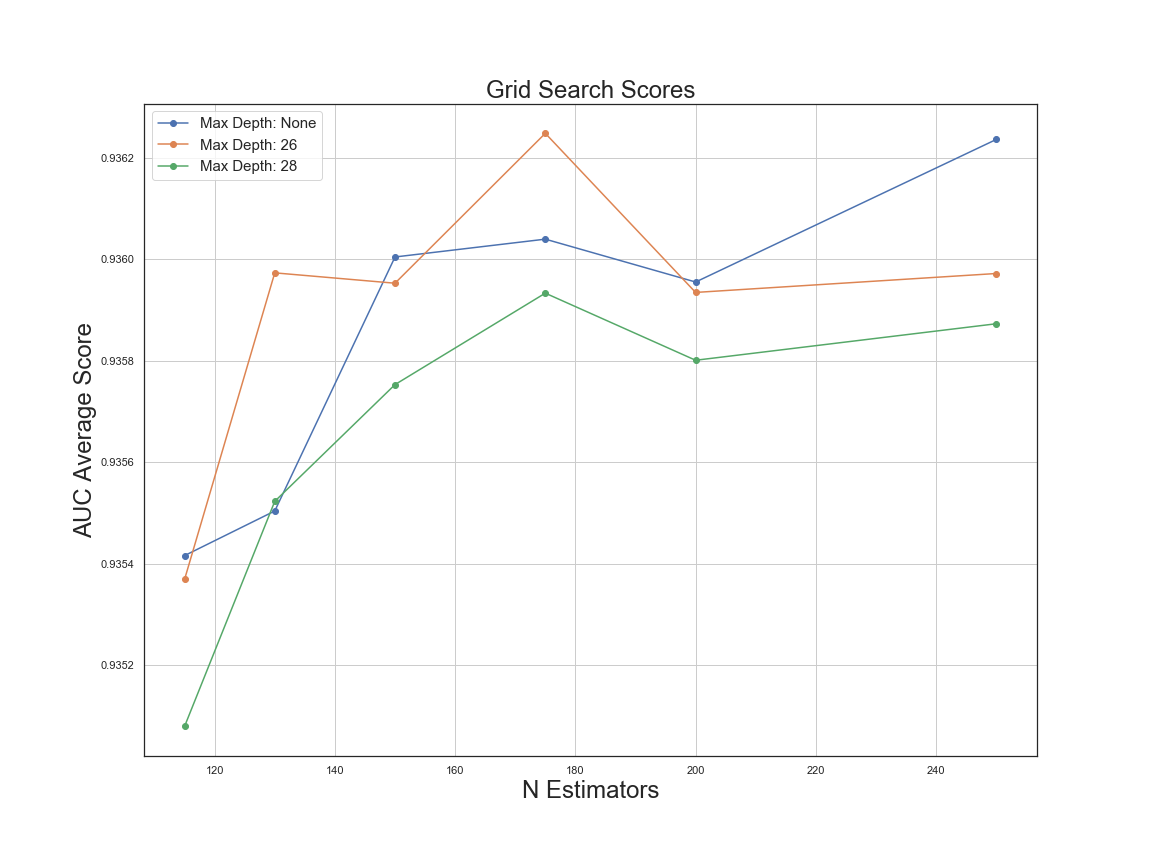
\includegraphics[width=\columnwidth]{chapter5/figure/gridSearch.png}
	\caption{Grid search results}
	\label{fig:grid_search}
\end{figure}
\begin{figure}[htp!]
	\centering
	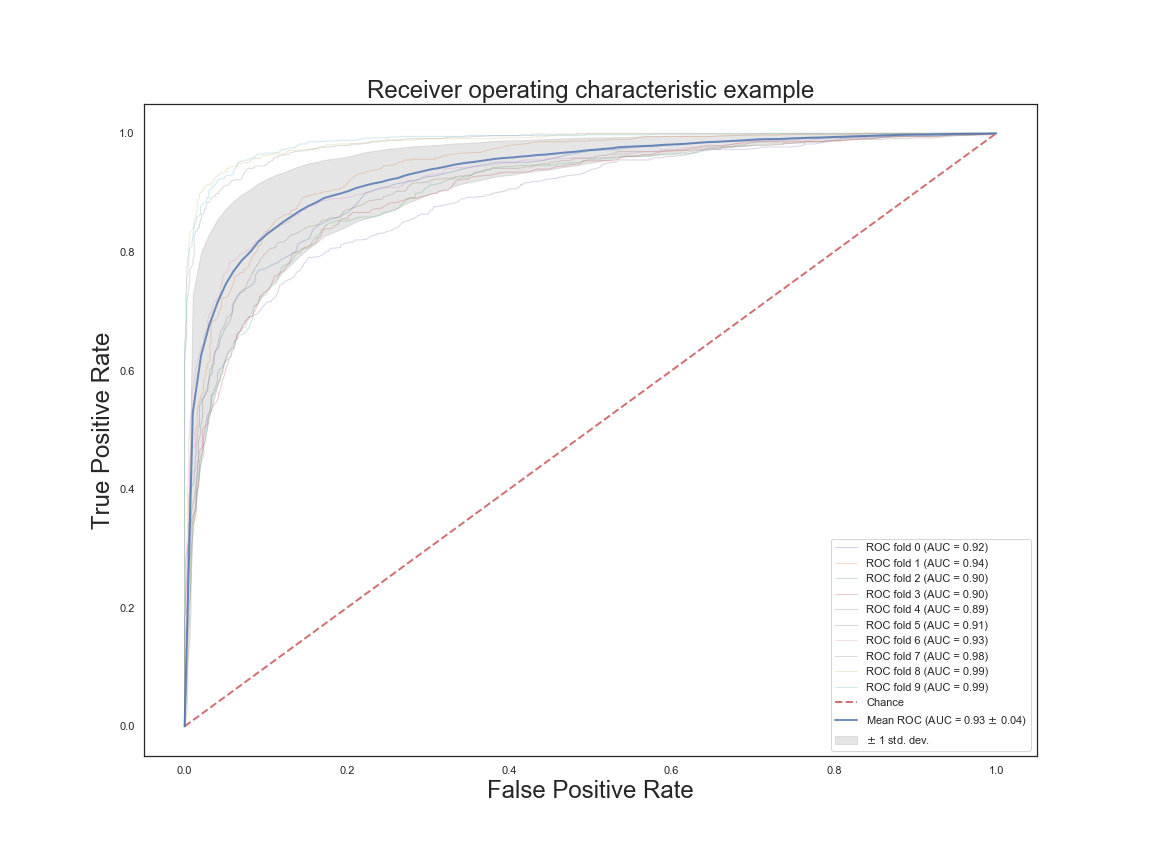
\includegraphics[width=\columnwidth]{chapter5/figure/auc.png}
	\caption{ROC curve}
	\label{fig:auc}
\end{figure}
As we can see in Figure \ref{fig:grid_search}, the AUC is increasing with the number of the estimators in the forest, but this trend slows down after 100 trees reached. We decided t stop at 175, which corresponds to a local maximum, in order to prefer a lighter model and a faster prediction time, which currently is set to 27ms.

The AUC obtained with this asset is equal to 0.936, as shown in Figure \ref{fig:auc}, which is a positive accomplishment, considering that it will be used only as support for the identification of humans among bots, but we didn't crafted specific features as the ones involved in the Botmoter project and we didn't have the same amount of data neither.

The final model has been fitted with the hole data, with this settings: \textit{ n\_estimators} = 175, \textit{max\_depth} = 26 and \textit{criterion} = 'entropy'.
Once we fitted the model, it was ready to be the first element of our solution pool.

\section{Text classifier}
\section{Stacking meta-classifier}
\subsection{Genetic algorithm}
\subsection{Logistic Regression}
\section{Validation}